\documentclass[12pt]{article}

\usepackage[a4paper,margin=2cm]{geometry}

\usepackage{amsmath}
\usepackage{amssymb}
\usepackage{mathtools}

\usepackage{listings}

\usepackage{booktabs} % For tables
\usepackage[table,xcdraw]{xcolor} % For table

\usepackage{parskip}

\usepackage{booktabs} % For tables
\usepackage[table,xcdraw]{xcolor} % For tables

\usepackage{enumerate}
\usepackage{enumitem}
\usepackage{tikz}
\usepackage{float}

\usepackage{nameref}

\usepackage{hyperref}
\usepackage{xcolor}

\definecolor{codegreen}{rgb}{0,0.6,0}
\definecolor{codegray}{rgb}{0.5,0.5,0.5}
\definecolor{codepurple}{rgb}{0.58,0,0.82}
\definecolor{backcolour}{rgb}{0.95,0.95,0.92}

\lstdefinestyle{mystyle}{
    backgroundcolor=\color{backcolour},
    commentstyle=\color{codegreen},
    keywordstyle=\color{magenta},
    numberstyle=\tiny\color{codegray},
    stringstyle=\color{codepurple},
    basicstyle=\ttfamily\footnotesize,
    breakatwhitespace=false,
    breaklines=true,
    captionpos=b,
    keepspaces=true,
    numbers=left,
    numbersep=5pt,
    showspaces=false,
    showstringspaces=false,
    showtabs=false,
    tabsize=2
}

\lstset{style=mystyle}

\DeclarePairedDelimiter\abs{\lvert}{\rvert}
\DeclarePairedDelimiter\Abs{\lVert}{\rVert}

\usepackage{fancyhdr}

\pagestyle{fancy}
\lhead{\today}
\chead{Exercise 03\\Algorithmic Foundations of Data Science}
\rhead{Fabian Grob\\Simon Michau\\Til Mohr}

\setlength{\headheight}{50pt}

\begin{document}

\section*{Exercise 1}
\begin{enumerate}[label= (\alph*)]
	\item	Using Theorem 3.6: With \(|\mathcal{H}| = 3^3 = 27\)
			\begin{align*}
				\Pr_{T ~ \mathcal{D}^m} &\left( \forall h \in \mathcal{H}: \abs{err_T(h) - err_D(h)} \leq \epsilon \right) > 1 - \delta \\
				\Pr_{T ~ \mathcal{D}^m} &\left( \forall h \in \mathcal{H}: \abs{err_T(h) - err_D(h)} \leq \epsilon \right) > 0.9 \\
				\Rightarrow &\delta = 0.1 \\\\
				m &\geq \frac{1}{2\epsilon^2} \log \left( \frac{2\abs{\mathcal{H}}}{\delta} \right) \\
				143 &\geq \frac{1}{2\epsilon^2} \log \left( \frac{2 \cdot 3^3}{0.1} \right) \\
				143 &\geq \frac{1}{2\epsilon^2} (\log(54) - \log(0.1)) \\
				143 &\geq \frac{1}{2\epsilon^2} (\log(54) - \log(0.1)) \\
				\epsilon^2 &\geq \frac{(\log(54) - \log(0.1))}{143 \dot 2} \\
				\abs{\epsilon} &\geq \sqrt{\frac{(\log(54) - \log(0.1))}{286}} \\
				\Rightarrow &\epsilon \geq \sqrt{\frac{(\log(54) - \log(0.1))}{286}} \\
				\Pr_{T ~ \mathcal{D}^m} &\left( \forall h \in \mathcal{H}: \abs{err_T(h) - err_D(h)} \leq \epsilon \right) > 0.9 \\
				\Pr_{T ~ \mathcal{D}^m} &\left( \forall h \in \mathcal{H}: \abs{0.03 - err_D(h)} \leq \sqrt{\frac{(\log(54) - \log(0.1))}{286}} \right) > 0.9 \\
				\Rightarrow &err_D(h) \leq 0.03 + \sqrt{\frac{(\log(54) - \log(0.1))}{286}} \simeq 0.208149 \simeq 0.21
			\end{align*}
	\item	Using Theorem 3.4:
			\begin{align*}
				\Pr_{T ~ \mathcal{D}^m} &\left( \forall h \in \mathcal{H}: \text{if $h$ is consistent with $T$, then } err_D(h) \leq \epsilon \right) 1 - \delta \\
				\Pr_{T ~ \mathcal{D}^m} &\left( \forall h \in \mathcal{H}: \text{if $h$ is consistent with $T$, then } err_D(h) \leq 0.01 \right) 0.9 \\
				\Rightarrow &\epsilon = 0.01, \delta = 0.1 \\\\
				m &\geq \frac{1}{\epsilon} \ln \left( \frac{\abs{\mathcal{H}}}{\delta} \right) \\
				m &\geq \frac{1}{0.01} \ln \left( \frac{3^3}{0.1} \right) \\
				m &\geq 100 (\ln(27) - \ln(0.1)) \simeq = 559.84 \\
				\Rightarrow &m \geq 560
			\end{align*}
\end{enumerate}

\section*{Exercise 2}
Using slide 3.26.
\begin{enumerate}[label=(\alph*)]
	\item	The dimension of the instance space is $l = a \cdot v$. Such a decision scheme can be described using $\abs{h}_{\Delta} \in O(n(\log n + \log l)) = O(n(\log n + \log (a \cdot v))) = O(n (\log n + \log a + \log v))$ bits.
	\item	$n=10, a = 5, v = 5$ ???????????????????
\end{enumerate}

\section*{Exercise 3}
\begin{enumerate}[label=(\alph*)]
	\item	The VC-Dimension is $3$. To prove this, let us prove some properties which every $Y$, that shatters $\mathcal{H}$, must hold.

			\textbf{Notation:}
			\begin{itemize}
				\item	$a_i, b_i \in \mathbb{R}, i \in \mathbb{N}$
				\item	$y_{i,j} \in Y , i,j \in \mathbb{N} \rightarrow y_{i,j} = (a_i, b_j)$ (analog for $y'_{i,j} \in Y'$)
			\end{itemize}

			\textbf{Property 1:}
			$$\neg \exists y_{i, j} \exists y_{i', j'} \exists y_{i'', j''} (a_i \neq a_{i'} \land a_i \neq a_{i''} \land a_{i'} \neq a_{i''} \land b_i \neq b_{i'} \land b_i \neq b_{i''} \land b_{i'} \neq b_{i''})$$
			\textit{In words: There cannot be 3 vectors in $Y$ that have neither their $a$ nor $b$ values in common.} \\
			Let's prove this be counterexample. \\
			Let $Y' = \{(a_1, b_1), (a_2, b_2), (a_3, b_3)\} \subseteq Y$. There exists no $h_{a,b} \in \mathcal{H}$, such that $Y' \subseteq S_{h_{a,b}}$. Therefore, $Y' = S_{h_{a,b}} \cap Y$ does not hold.

			\textbf{Property 2:}
			$$\neg \exists y_{i, j} \exists y_{i', j'} \exists y_{i'', j''} (y_{i,j} \neq y_{i',j'} \land y_{i,j} \neq y_{i'',j''} \land y_{i',j'} \neq y_{i'',j''}) \land ((a_i = a_{i'} \land a_i = a_{i''}) \lor (b_i = b_{i'} \land b_i = b_{i''}))$$
			\textit{In words: There cannot be 3 vectors in $Y$ that have their $a$ or $b$ values in common.} \\
			Let's prove this be counterexample. \\
			Let $Y' = \{(a_1, b_1), (a_1, b_2)\} \subseteq \{(a_1, b_1), (a_1, b_2), (a_1, b_3)\} \subseteq Y$ (analog when the $b$-components are equal). Then there exists no $h_{a,b} \in \mathcal{H}$ so that $Y' \subseteq S_{h_{a,b}}$ but $(a_1, b_3) \not\in S_{h_{a,b}}$. This is true, since the only functions $h_{a,b}$ with $Y' \subseteq S_{h_{a,b}}$ are where $a = a_1$, thus also $(a_1, b_3) \not\in S_{h_{a,b}}$, which is a contradiction.

			\textbf{Property 3:}
			$$\neg \exists y_{i, j} \exists y_{i', j'} \exists y_{i'', j''} (y_{i,j} \neq y_{i',j'} \land y_{i,j} \neq y_{i'',j''} \land y_{i',j'} \neq y_{i'',j''}) \land (a_i = a_{i'} \land b_{i'} = b_{i''})$$
			\textit{In words: There cannot be a vector containing of an $a$-component that also exists in another vector and a $b$-component that also exists in another vector.} \\
			Let's prove this be counterexample. \\
			Let $Y' = \{(a_1, b_2)\} \subseteq \{(a_1, b_1), (a_1, b_2), (a_2, b_2)\} \subseteq Y$.
			For all $h_{a,b} \in \mathcal{H}$ with $Y' \subseteq S_{h_{a,b}}$ $a=a_1 \lor b=b_2$ must hold. However, for such $h_{a,b}$ $(a_1, b_1) \in S_{h_{a,b}}$ or $(a_2, b_2) \in S_{h_{a,b}}$ would also hold. This is a contradiction.

			Thus, the only valid form of $Y$ must be (or analog when two $b$-components are equal):
			$$Y \coloneqq \{(a_1, b_1), (a_1, b_2), (a_2, b_2)\}, a_1 \neq a_2 \land b_1 \neq b_2 \land b_1 \neq b_3 \land b_2 \neq b_3$$
			We can prove that $Y$ shatters $\mathcal{H}$:
			\begin{itemize}
				\item	$Y' = \emptyset$: \\
						We can use $h_{a_0, b_0}$ with $a_0 \not\in \{a_1, a_2\}, b_0 \not\in \{b_1, b_2, b_3\}$. Thus, $Y \not\in S_{h_{a_0,b_0}}$. So, $Y' = \emptyset = S_{h_{a_0,b_0}} \cap Y$.
				\item	$Y' = \{(a_1, b_i)\}$, $i \in \{1,2\}$: \\
						We can use $h_{a_0, b_i}$ with $a_0 \not\in \{a_1, a_2\}$. Thus, $Y' = \emptyset = S_{h_{a_0,b_i}} \cap Y$.
				\item	$Y' = \{(a_2, b_3)\}$: \\
						We can use $h_{a_2, b_3}$. Thus, $Y' = \emptyset = S_{h_{a_0,b_i}} \cap Y$.
				\item	$Y' = \{(a_1, b_1), (a_1, b_2)\}$: \\
						We can use $h_{a_1, b_1}$. Thus, $Y' = \emptyset = S_{h_{a_0,b_i}} \cap Y$.
				\item	$Y' = \{(a_1, b_i), (a_2, b_3)\}$, $i \in \{1,2\}$: \\
						We can use $h_{a_2, b_i}$. Thus, $Y' = \emptyset = S_{h_{a_0,b_i}} \cap Y$.
				\item	$Y' = Y$: \\
						We can use $h_{a_1, b_3}$. Thus, $Y' = \emptyset = S_{h_{a_0,b_i}} \cap Y$.
			\end{itemize}
			So, the VC-Dimension is at least $3$. Let's now prove, that no $Y$ with $\abs{Y} > 3$ shatters $\mathcal{H}$.

			For now, let $Y$ be $Y \coloneqq \{(a_1, b_1), (a_1, b_2), (a_2, b_2)\}$, $a_1 \neq a_2 \land b_1 \neq b_2 \land b_1 \neq b_3 \land b_2 \neq b_3$ (which we proved was the only valid form of $Y$ with $\abs{Y} = 3$). We can now try to add any $y_{i,j}$ to $Y$:
			\begin{itemize}
				% a_1
				\item	Let's try to add $y_{1,j} = (a_1, b_j)$, $j \in \mathbb{N}$. This would violate \textbf{Property 1}. Thus, we cannot add any such $y_{1,j}$.

				% a_2
				\item	Let's try to add $y_{2,j} = (a_2, b_j)$, $j \in \mathbb{N}$. Since $(a_2, b_3) \in Y$, $b_j \in \mathbb{R}\setminus\{b_3\}$. Then the condition in the remark would not hold for $Y' = Y$. Thus, we cannot add any such $y_{2,j}$.

				% a_3
				\item	Let's try to add $y_{3,4} = (a_3, b_4)$, $a_3 \in \mathbb{R}\setminus\{a_1, a_2\}$, $b_4 \not\in \{b_1, b_2, b_3\}$. This would violate \textbf{Property 1}. Thus, we cannot add any such $y_{3,4}$.
				\item	Let's try to add $y_{3,j} = (a_3, b_j)$, $j \in \{1,2\}$, $a_3 \in \mathbb{R}\setminus\{a_1, a_2\}$. Then, we cannot find any $h_{a,b} \in \mathcal{H}$ for $Y' = Y$, so that the condition in the remark holds. Thus, we cannot add any such $y_{3,j}$
				\item	Let's try to add $y_{3,j} = (a_3, b_3)$, $a_3 \in \mathbb{R}\setminus\{a_1, a_2\}$. Then, for $Y' = \{(a_1, b_2), (a_2,b_3), (a_3, b_3)\}$ we cannot find any $h_{a,b} \in \mathcal{H}$, for which $Y' \subseteq S_{h_{a,b}}$ but $(a_1, b_1) \not\in S_{h_{a,b}}$. Thus, we cannot add any such $y_{3,j}$.
			\end{itemize}
			So, we cannot add any element to $Y$. Thus, all $Y$ that shatter $\mathcal{H}$ must be at most $\abs{Y} \leq 3$. Therefore, the VC Dimension is $3$.
	\item	The VC-Dimension is $\infty$. \\
			Let be $Y \subseteq \mathfrak{X} = \Sigma^*$. For any $Y' \subseteq Y$ we can choose $L \coloneqq Y'$. Thus, $Y' = S_{h_L}$, so also $S_{h_L} \subseteq Y$. So $Y \cap S_{h_L} = S_{h_L} = Y'$. So $Y$ can also be infinite in size.
\end{enumerate}

\section*{Exercise 4}
\begin{enumerate}[label= (\alph*)]
	\item See \refname{appendix} for code.
        \lstinputlisting{code/exercise_04_output.txt}
    \item No, the weights are always the same. This is because the loss matrix does not change throughout the algorithm, so the loss is always the same.
        If all the events still happen in the sequence, only in a different order, this won't have an effect as the loss will still be included in the updated weight.
\end{enumerate}

\section*{Exercise 5}
\begin{enumerate}[label=(\alph*)]
	\item See \refname{appendix} for code.
        \lstinputlisting{code/exercise_05_output.txt}
    \item \(w_1^{(4)}\) and \(w_3^{(4)}\) are different because with \(\gamma = 0.5\) we put a certain weight on exploration.
        Therefore, even with the same reward, different actions can have different weights as \(\gamma\) is part of the weight updating calculation.
\end{enumerate}

\section*{Exercise 6}
\begin{enumerate}[label= (\alph*)]
    \item   \begin{enumerate}[label= (\roman*)]
                \item  \begin{figure}[H]
                            \centering
                            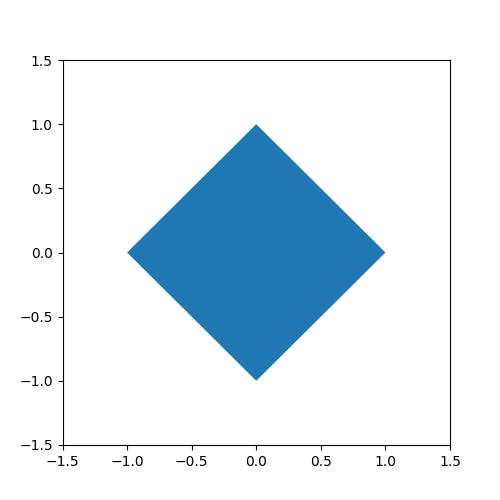
\includegraphics[width=3.5in]{code/exercise_06_a.png}
                        \end{figure}
                \item The shape of \(B^3_1 \subset \mathcal{R}^3\) would look like a octahedron with the same edge length ($\sqrt{2}$).
            \end{enumerate}
    \item \(|diag(B^2_1)| = 2 \xRightarrow{\text{Pythagoras}} \text{edge length of }B^2_1 = \sqrt{2} \Rightarrow vol(B^2_1) = \sqrt{2}^2 = 2\) \\
        \(vol(B^3_1) = \frac{1}{3}\sqrt{2}a^3\) with $a$ being the edge length of the octahedron \(\Rightarrow vol(B^3_1) = \frac{1}{3}\sqrt{2}^4 = \frac{1}{3}4 = \frac{4}{3} \simeq  1.33\)\\
        A more general formula for the volume \(vol(B^l_1)\) is \(vol(B^l_1) = \frac{2^l}{l!}\) (cmp. this \href{https://doi.org/10.2307/30044198}{paper}).\\
        Using \(l = 1, 2\) yields the same results.
    \item
        \begin{align*}
            &\lim_{l\rightarrow\inf}{\text{vol}(B^l_1) = \frac{2^l}{l!}}\\
            &\Rightarrow \lim_{l\rightarrow\inf}{\text{vol}(B^l_1)} = \frac{2}{1}\cdot \frac{2}{2}\cdot \frac{2}{3}\cdot \dotsb \cdot\frac{2}{l-1}\cdot \frac{2}{l}\\
            & \leq 2 \cdot \frac{2}{l}  = \frac{4}{l} \\
            &\Rightarrow \lim_{n\rightarrow\inf}{\frac{4}{l}} = 0
        \end{align*}

\end{enumerate}

\section*{Appendix}\label{appendix}
\subsection*{Code for Exercise 4}
\lstinputlisting[language=Python]{code/exercise_04.py}
\subsection*{Code for Exercise 5}
\lstinputlisting[language=Python]{code/exercise_05.py}
% \bibliographystyle{plainnat}
% \bibliography{\jobname}

\end{document}